\begin{titlepage}
    \centering
    
    \scshape

    \vspace*{-1.5cm}
    
    % Título
    
    \rule{\textwidth}{1.6pt}\vspace*{-\baselineskip}\vspace*{2pt}
    \rule{\textwidth}{0.4pt}
    
    \vspace{0.7\baselineskip}
    
    \Huge{Como Jogar Go}\\
    \vspace*{10pt}
    \LARGE{Uma Introdução Concisa}
    
    \vspace{0.275\baselineskip}
    
    \rule{\textwidth}{0.4pt}\vspace*{-\baselineskip}\vspace{3.2pt}
    \rule{\textwidth}{1.6pt}

    % Imagem
    
    \vspace*{.4cm}

    \begin{figure}[h]
        \centering
        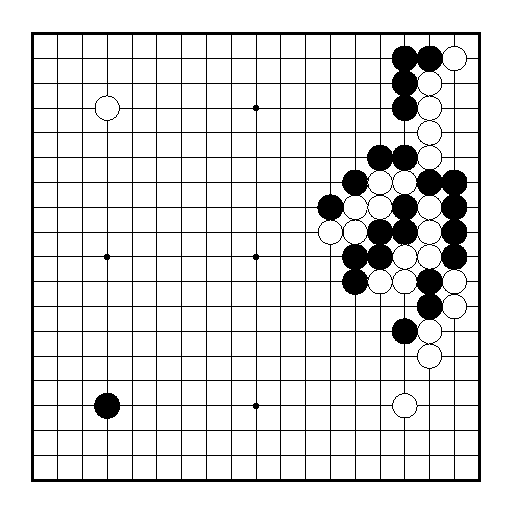
\includegraphics[scale=.9]{Ancient Game Nao Numerado}
    \end{figure}

    % Autores
    
    \vspace*{0.2cm}

    \large{por}

    \vspace*{0.125cm}

    \Large{Richard Bozulich}\\
    \normalsize{\&}\\
    \Large{James Davies}

    % Tradutor
    
    \vfill

    \large{traduzido por}

    \vspace*{0.125cm}

    \Large{Philippe Fanaro}
    
    % Editora e Logos

    \vfill
    
    \large{Kiseido Publishing Company}

    \vspace*{0.25cm}
    
    \large{Fanaro.io}
\end{titlepage}